\documentclass[a4paper,12pt]{article}
% Package to make citations superscrit with brackets
\usepackage[super,square]{natbib}
% Package to change margin size
\usepackage{anysize}
\usepackage{comment}
\usepackage{amsmath}
\marginsize{2cm}{2cm}{1cm}{2cm}
% Package to make headers
\usepackage{fancyhdr}
\usepackage{circuitikz}
\renewcommand{\headrulewidth}{0pt}
\usepackage{soul}
\usepackage[section]{placeins}
% Colors for the references links
\usepackage[dvipsnames]{xcolor}
% Package to link references
\usepackage{hyperref}
\usepackage{graphicx}
\hypersetup{
    colorlinks=true,
    linkcolor=black,
    citecolor=CadetBlue,
    filecolor=CadetBlue,      
    urlcolor=CadetBlue,
}
% Package for lorem ipsum
\usepackage{lipsum}
% Package for multicolumn
\usepackage{multicol}
% Package for removing paragraph identations
\usepackage{parskip}
\setlength\columnsep{18pt}
% Sets bastract
\renewenvironment{abstract}
 {\par\noindent\textbf{\abstractname}\ \ignorespaces \\}
 {\par\noindent\medskip}



 
\begin{document}
% Makes header
\pagestyle{fancy}
\thispagestyle{empty}
\fancyhead[R]{\textit{EE1200}}
\fancyhead[L]{}
% Makes footnotes with an asterisk
\renewcommand*{\thefootnote}{\fnsymbol{footnote}}
\begin{center}
\Large{\textbf{Experiment 04}}
\vspace{0.4cm}
\normalsize
\\ Aditya Tripathy - ee24btech11001, Durgi Swaraj Sharma - ee24btech11018\\
\medskip
\normalsize
\end{center}
{\color{gray}\hrule}
\vspace{0.4cm}
\begin{abstract}
In Experiment-04, we try to capture LC oscillations.
\end{abstract}
{\color{gray}\hrule}
\medskip
\section{Objective}
To study the response of a series RLC circuit with a precharged capacitor.

\section{Apparatus}
\begin{itemize}
\item LM 358
\item Two 10$k\Omega$ resistors
\item Two PN - junction diodes
\item Oscilloscope
\item Function Generator
\end{itemize}
\section{Theory}

The half wave rectifier implemented with a series connection of a resistor and a PN-junction diode is suboptimal in its working due to the threshold voltage required for the flow of current in the 
positive half cycle of the input wave. 

To implement a better half wave rectifer free from the above mentioned problem we use the following circuit which makes use of an op-amp and a couple of diodes commonly known as a precision half wave
rectifier or a superdiode.

\begin{figure}[!ht]
\centering
\resizebox{0.5\textwidth}{!}{%
\begin{circuitikz}
\tikzstyle{every node}=[font=\normalsize]

\draw (11.5,15.5) node[op amp,scale=1, yscale=-1 ] (opamp2) {};
\draw (opamp2.+) to[short] (10,16);
\draw  (opamp2.-) to[short] (10,15);
\draw (12.7,15.5) to[short](13,15.5);
\draw (10,15) to[R] (7.25,15);
\draw (9.5,15) to[short] (9.5,10.5);
\draw (9.5,12.25) to[D] (13.25,12.25);
\draw (13,15.5) to[D] (16,15.5);
\draw (13.25,12.25) to[short] (13.25,15.5);
\draw (9.5,10.5) to[R] (16,10.5);
\draw (10,16) to (6,16) node[ground]{};
\node [font=\normalsize] at (12.75,10) {$R_f$};
\node [font=\normalsize] at (11.5,11.75) {$D_1$};
\node [font=\normalsize] at (14.5,14.75) {$D_2$};
\node [font=\normalsize] at (8.5,14.5) {$R_1$};
\node [font=\normalsize] at (6.75,15) {V(t)};
\node [font=\normalsize] at (18.75,15.5) {$V_{out}$};
\draw (16,10.5) to[short] (16,15.5);
\draw (16,15.5) to[short] (18.25,15.5);
\node [font=\normalsize] at (13.25,15.75) {$V_o$};
\draw (11.5,15.5) node[op amp,scale=1, yscale=-1 ] (opamp2) {};
\draw (opamp2.+) to[short] (10,16);
\draw  (opamp2.-) to[short] (10,15);
\draw (12.7,15.5) to[short](13,15.5);
\draw (11.5,15.5) node[op amp,scale=1, yscale=-1 ] (opamp2) {};
\draw (opamp2.+) to[short] (10,16);
\draw  (opamp2.-) to[short] (10,15);
\draw (12.7,15.5) to[short](13,15.5);
\draw (11.5,15.5) node[op amp,scale=1, yscale=-1 ] (opamp2) {};
\draw (opamp2.+) to[short] (10,16);
\draw  (opamp2.-) to[short] (10,15);
\draw (12.7,15.5) to[short](13,15.5);
\node [font=\normalsize] at (9.5,15.25) {$V_b$};
\end{circuitikz}
}%

\caption{Precision Rectifier}
\end{figure}

Initially all voltages are at 0V. When $V(t) > 0$, $V_o$ will also become positive. Thus, the flow of current will be as shown:
\begin{figure}[!ht]
\centering
\resizebox{0.5\textwidth}{!}{%
\begin{circuitikz}
\tikzstyle{every node}=[font=\normalsize]

\draw (11.5,15.5) node[op amp,scale=1, yscale=-1 ] (opamp2) {};
\draw (opamp2.+) to[short] (10,16);
\draw  (opamp2.-) to[short] (10,15);
\draw (12.7,15.5) to[short](13,15.5);
\draw (10,15) to[R] (7.25,15);
\draw (9.5,15) to[short] (9.5,10.5);
\draw (9.5,12.25) to[D] (13.25,12.25);
\draw (13,15.5) to[D] (16,15.5);
\draw (13.25,12.25) to[short] (13.25,15.5);
\draw (9.5,10.5) to[R] (16,10.5);
\draw (10,16) to (6,16) node[ground]{};
\node [font=\normalsize] at (12.75,10) {$R_f$};
\node [font=\normalsize] at (11.5,11.75) {$D_1$};
\node [font=\normalsize] at (14.5,14.75) {$R_2$};
\node [font=\normalsize] at (8.5,14.5) {$R_1$};
\node [font=\normalsize] at (6.75,15) {V(t)};
\node [font=\normalsize] at (18.75,15.5) {$V_{out}$};
\draw (16,10.5) to[short] (16,15.5);
\draw (16,15.5) to[short] (18.25,15.5);
\node [font=\normalsize] at (13.25,15.75) {$V_o$};
\draw (11.5,15.5) node[op amp,scale=1, yscale=-1 ] (opamp2) {};
\draw (opamp2.+) to[short] (10,16);
\draw  (opamp2.-) to[short] (10,15);
\draw (12.7,15.5) to[short](13,15.5);
\draw (11.5,15.5) node[op amp,scale=1, yscale=-1 ] (opamp2) {};
\draw (opamp2.+) to[short] (10,16);
\draw  (opamp2.-) to[short] (10,15);
\draw (12.7,15.5) to[short](13,15.5);
\draw (11.5,15.5) node[op amp,scale=1, yscale=-1 ] (opamp2) {};
\draw (opamp2.+) to[short] (10,16);
\draw  (opamp2.-) to[short] (10,15);
\draw (12.7,15.5) to[short](13,15.5);
\draw [->, >=Stealth] (7.5,13.75) -- (9.25,13.75);
\draw [->, >=Stealth] (9,13.25) -- (9,12.25);
\draw [->, >=Stealth] (9.75,12.75) -- (12.5,12.75);
\draw [->, >=Stealth] (13,13.25) -- (13,15);
\draw [->, >=Stealth] (12.5,15) -- (12,15);
\end{circuitikz}
}%
\caption{Current flow for positive half cycle}
\end{figure}
\newline
\newline
\newline
It is evident that the voltage at the $V_{out}$ is zero since the voltages at $t=0$ were all zero. 
\newline
When the input voltage is negative, the flow of current will be as follows:

\begin{figure}[!ht]
\centering
\resizebox{0.5\textwidth}{!}{%
\begin{circuitikz}
\tikzstyle{every node}=[font=\normalsize]

\draw (11.5,15.5) node[op amp,scale=1, yscale=-1 ] (opamp2) {};
\draw (opamp2.+) to[short] (10,16);
\draw  (opamp2.-) to[short] (10,15);
\draw (12.7,15.5) to[short](13,15.5);
\draw (10,15) to[R] (7.25,15);
\draw (9.5,15) to[short] (9.5,10.5);
\draw (9.5,12.25) to[D] (13.25,12.25);
\draw (13,15.5) to[D] (16,15.5);
\draw (13.25,12.25) to[short] (13.25,15.5);
\draw (9.5,10.5) to[R] (16,10.5);
\draw (10,16) to (6,16) node[ground]{};
\node [font=\normalsize] at (12.75,10) {$R_f$};
\node [font=\normalsize] at (11.5,11.75) {$D_1$};
\node [font=\normalsize] at (14.5,14.75) {$D_2$};
\node [font=\normalsize] at (8.5,14.5) {$R_1$};
\node [font=\normalsize] at (6.75,15) {V(t)};
\node [font=\normalsize] at (18.75,15.5) {$V_{out}$};
\draw (16,10.5) to[short] (16,15.5);
\draw (16,15.5) to[short] (18.25,15.5);
\node [font=\normalsize] at (13.25,15.75) {$V_o$};
\draw (11.5,15.5) node[op amp,scale=1, yscale=-1 ] (opamp2) {};
\draw (opamp2.+) to[short] (10,16);
\draw  (opamp2.-) to[short] (10,15);
\draw (12.7,15.5) to[short](13,15.5);
\draw (11.5,15.5) node[op amp,scale=1, yscale=-1 ] (opamp2) {};
\draw (opamp2.+) to[short] (10,16);
\draw  (opamp2.-) to[short] (10,15);
\draw (12.7,15.5) to[short](13,15.5);
\draw (11.5,15.5) node[op amp,scale=1, yscale=-1 ] (opamp2) {};
\draw (opamp2.+) to[short] (10,16);
\draw  (opamp2.-) to[short] (10,15);
\draw (12.7,15.5) to[short](13,15.5);
\draw [->, >=Stealth] (9.25,14) -- (7,14);
\draw [->, >=Stealth] (9,10.75) -- (9,13.75);
\draw [->, >=Stealth] (15.75,11) -- (10,11);
\draw [->, >=Stealth] (11.75,16.25) -- (16,16.25);
\draw [->, >=Stealth] (16.75,15.25) -- (16.75,10.5);
\node [font=\normalsize] at (9.5,15.25) {$V_b$};
\end{circuitikz}
}
\caption{Current flow for negative half cycle}
\end{figure}
The voltage at $V_{out}$ will approximately be equal to
\begin{align}
  V_{out} \approx \frac{-R_f}{R_1}V(t)
\end{align}
\newline
The advantage of the superdiode is that for the current to start flowing, the input voltage need
to be close to ratio of threshold voltage and open loop gain(a very large number)
\begin{align}
  V(t) \approx \frac{V_{th}}{A}, \text{where A = open loop gain}
\end{align}
as opposed to the threshold voltage in the resistor-diode-only approach. Thus a superdiode can be used to rectify signals of amplitude $\approx 100mV$.
\section{Procedure}
\begin{enumerate}
\item Connections
\begin{itemize}
\item Connect the circuit as shown in Figure 1.
\item Connect $V_+$ to $15 V$ and $V_-$ to $-15 V$ 
\item Connect the probe of the oscilloscope across the common ground and output pin of the LM358.
\end{itemize}
\end{enumerate}

\section{Response captured}
\begin{figure}[!htb]
  {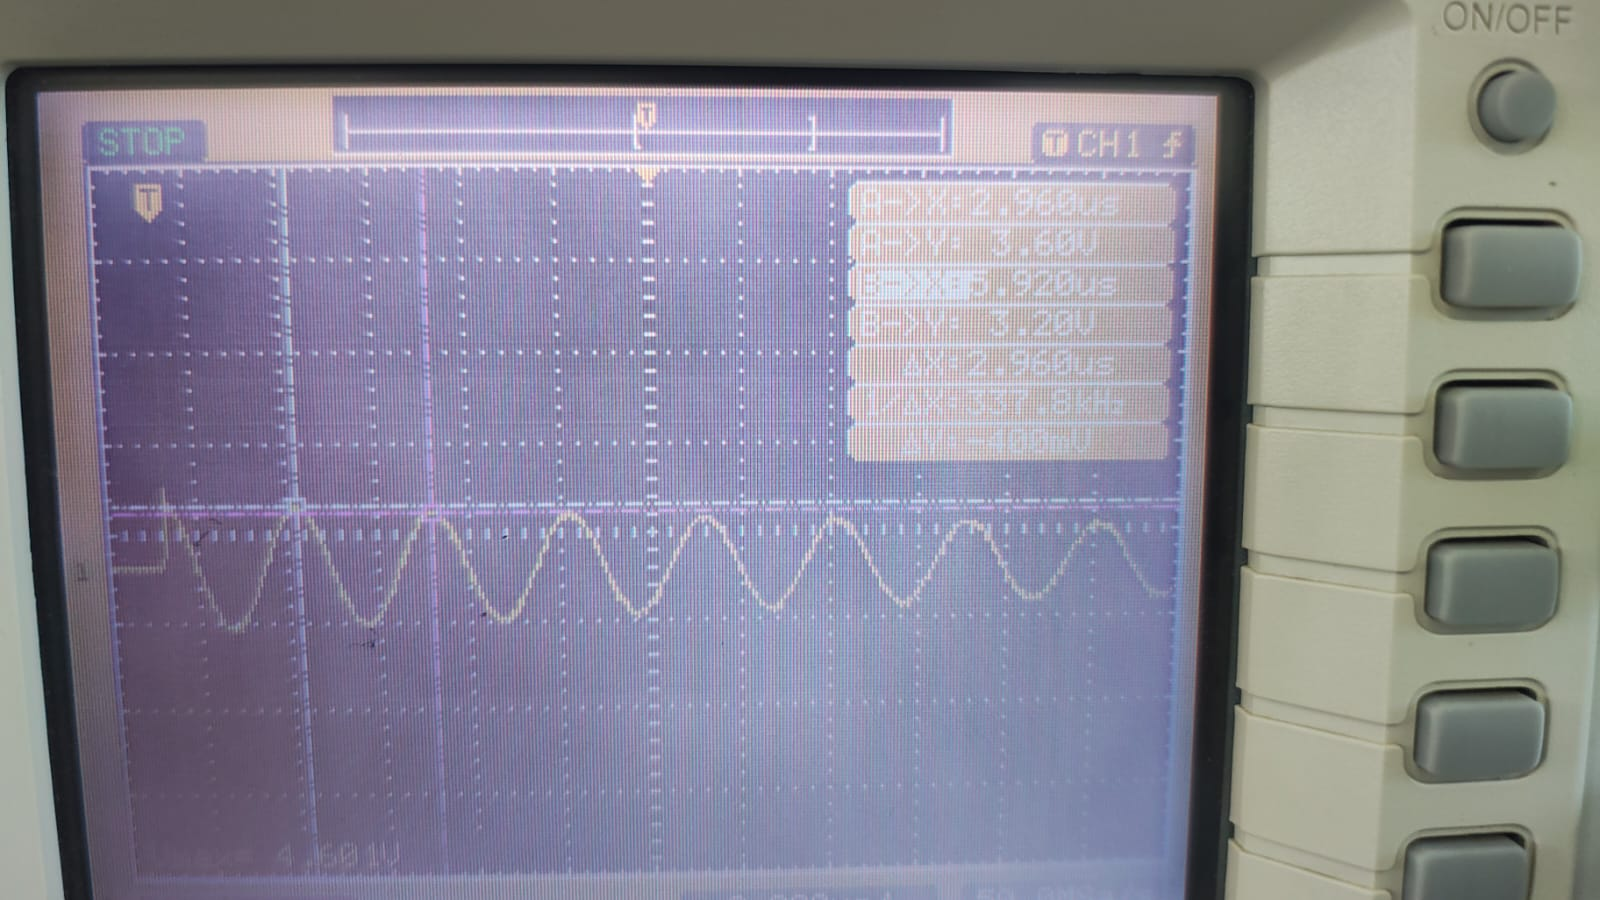
\includegraphics[width=0.5\columnwidth]{fig1.jpeg}}
  \caption{Response for resitor-diode-only circuit}
\end{figure}
\begin{figure}[!htb]
  {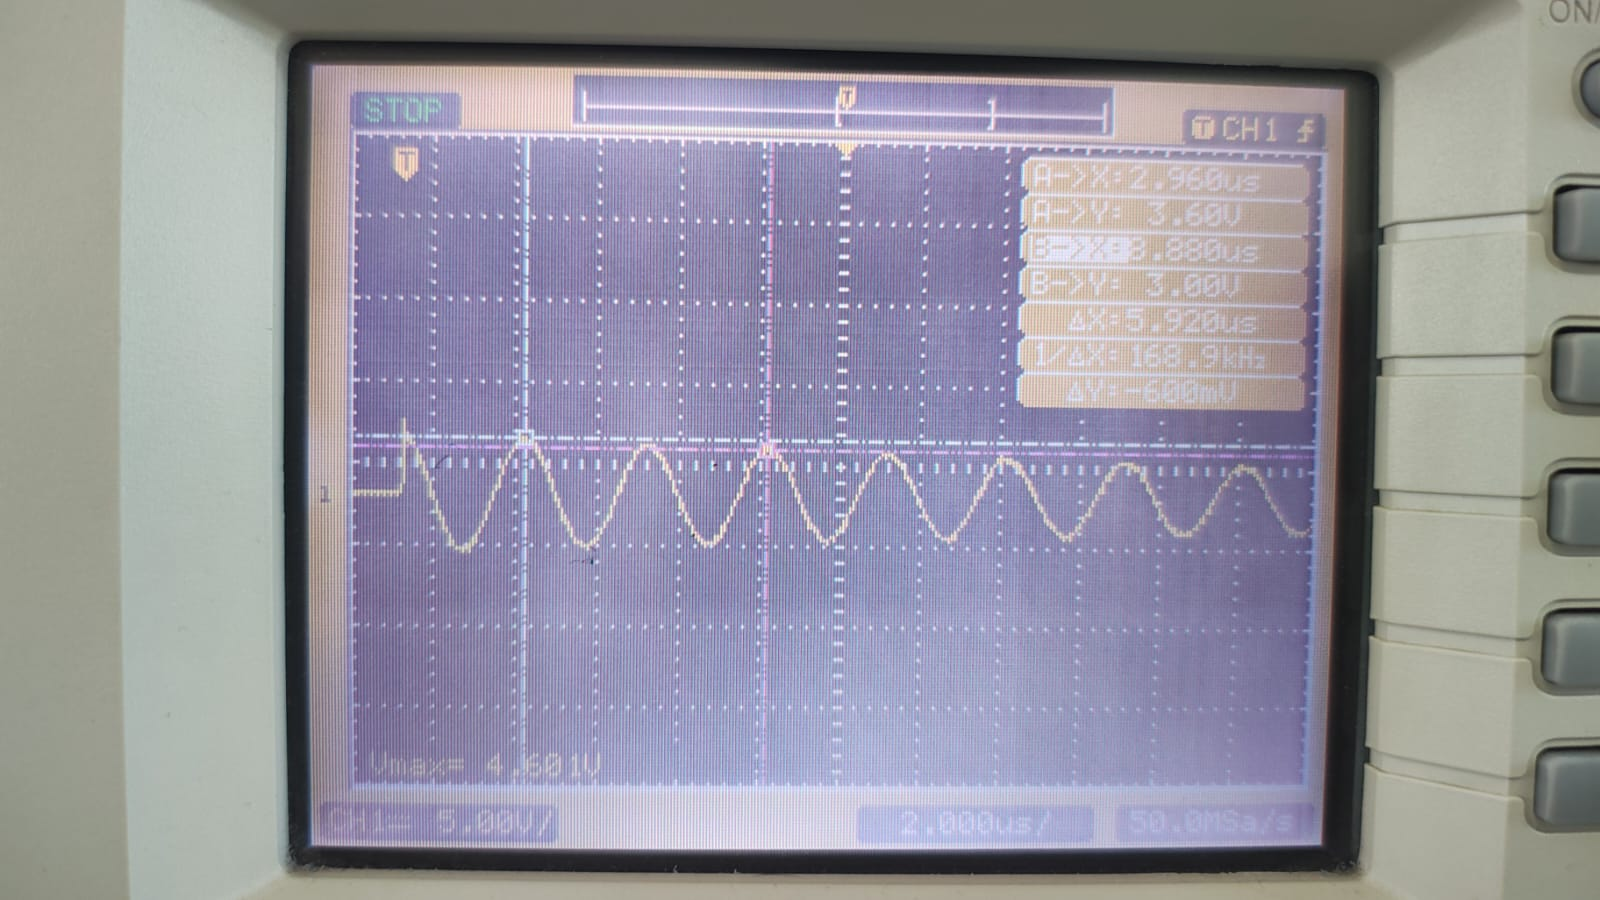
\includegraphics[width=0.5\columnwidth]{fig2.jpeg}}
  \caption{Response for superdiode circuit}
\end{figure}

\end{document}
